\section{Lezione 2016-10-06}
\subsection{TODO}
% Insert what you need. Any row is associated with the improvment or mistake
% arise. In the first column you can insert what you should resolve or change,
% instead in the second column you may put the section where to apply some
% modification.
\begin{table}[ht]
\begin{center}
\begin{tabular}{|p{\textwidth}|c|}
\hline
\multicolumn{1}{|c|}{\textbf{Miglioramento}} & \textbf{Sezione} \\ \hline
Nella conversione da DFA a grammatica lineare, $\epsilon$ della prima produzione
non \`e chiaro se \`e dovuto al fatto che sia stato iniziale o accettate &
\ref{sec:grammatica_lineare_destra} \\ \hline
Definire meglio il termine \textit{supremum} &
\ref{sec:theorem_fixed_point} \\ \hline
Leggere la sezione 3.9 del \textit{Dragon Book} per vedere come ottenere un
DFA dalla RE senza costruire l'NFA assiociato & \\ \hline
Chidere spiegazioni sul fatto del perch\'e la grammatica non sia $LL(1)$ &
\href{http://www.di.unipi.it/~andrea/Didattica/PLP-16/SLIDES/PLP-2016-07.pdf}{
slide 22
} \\ \hline
Inserire il link all'algoritmo \textit{match} degli appunti precedenti &
\ref{par:if_terminal} \\ \hline
Chiedere come \`e possibile determinale la produzione con cui fare il confronto
nell'algoritmo fig.\ref{img:PPP}. Inoltre se il non-terminale ha produzioni
multiple come si eseguirebbe il confronto. &
\ref{par:if_non-terminal} \\ \hline
Chiedere come nel \textit{Phrase-level Recovery} come si decide dove posizionare
l'azione di correzzione & \ref{sec:phrase-level_recovery} \\ \hline
\end{tabular}
\end{center}
\caption{Tabella miglioramenti}
\label{tab:tab_todo}
\end{table}


\subsection{Dal DFA ad una espressione regolare}
A volte \`e pi\`u intuitivo scrivere direttamente l'automa a stati finiti che
accetta le stringhe di un linguaggio piuttosto di comporre l'espressione
regolare associata. Si \`e vista la relazione che lega le RE-NFA-DFA, con l'
aggiunta della \textit{Right-linear Grammars} \`e possibile definire la
relazione da DFA-RE.

\begin{figure}[H]
\begin{center}
\includegraphics[scale=0.5]{res/image/relations}
\end{center}
\caption{Relazione rappresentazioni di un linguaggio}
\label{img:relations}
\end{figure}

\subsection{Grammatica lineare destra}
\label{sec:grammatica_lineare_destra}
\begin{definition}[Right-linear grammar]
In una grammatica lineare destra ogni produzione \`e della forma:
$A \to wB \text{ o } A \to w \ (w \in T^*)$.
\end{definition}

Dato un DFA $D = (Q,\Sigma, \delta, q_0, F)$ i passaggi per convertirla in una
\textit{Right-linear Grammar} sono la creazioni della forma:
$$q \to t_1\delta(q,t_1) \mid ... \mid t_n\delta(q,t_n) \quad \forall q \in Q$$
dove $t_i$ sono le etichette degli archi \textbf{entranti} in $q$. Nel caso
$q \in F$ (ovvero stato finale) si aggiunge la $\epsilon$\textit{-transition}
nella produzione\footnote{Supposizione! Da confermare}. La costruzione vale
anche per NFA. \`E anche possibile utilizzarla per convertire una qualsiasi
grammatica lineare destra in NFA (le produzioni dovrebbero essere trasformate
introducendo nuovi non-terminali).

\begin{figure}[H]
\begin{center}
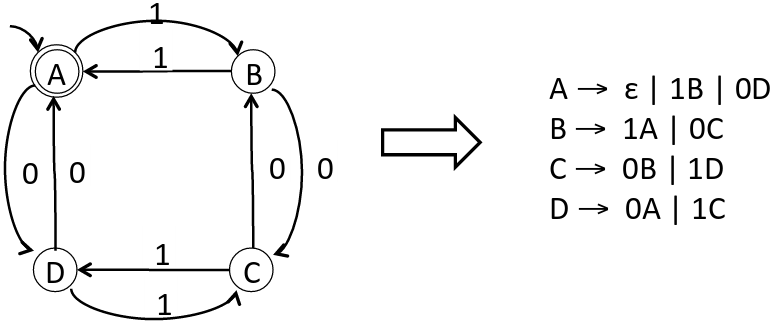
\includegraphics[scale=0.5]{res/image/from_dfa_to_re}
\end{center}
\caption{Esempio da DFA a RE}
\label{img:from_dfa_to_re}
\end{figure}

\subsubsection{Teorema del punto fisso}
\label{sec:theorem_fixed_point}
Prima di esporre il teorema \`e necessario introdurre il concetto di
\textbf{ordine completo parziale}:
\begin{definition}[CPO - Complete Partial Order]
Un ordine completo parziale \`e un ordine parziale con almeno $\perp$ e tale
che ogni catena di incrementi\footnote{$a < b < ... < z < ...$} abbiano un
supremum.
\end{definition}

Adesso esponiamo il teorema del punto fisso di Kleene:
\begin{definition}[Kleene fixed-point thorem]
Ogni funzione continua $F$ su un ordine completo parziale (CPO) ha almeno un
punto fisso, il quale \`e il supremum della catena:
$$F(\perp) \leq F(F(\perp)) \leq ... \leq F^n(\perp) \leq ...$$
\end{definition}

\subsubsection{Una CFG come funzione sul CPO dei linguaggi}
Un linguaggio su $\Sigma$ forma un ordine completo parziale sotto un'insieme di
inclusioni. Una \textit{context-free grammar} definisce una funzione continua
sui linguaggi\footnote{nelle slide si riferisce alla sequenza}
\begin{align*}
&A \to a | bA & F(L)=\{a\} \cup \{bw \mid w \in L\}
\end{align*}
Il linguaggio generato dalla grammatica \`e il minimo punto fisso della funzione
associata
$$
\emptyset \subset \{a\} \subset \{a,b\} \subset \{a,ba,bba\} \subset ...
\subset \{b^na \mid n \geq 0\}
$$
nel caso di grammatiche lineari destre noi possiamo descrivere il minimo punto
fisso come un'espressione regolare
$$Lang(A)=b^*a$$

Qui sotto e' un esempio di come dalla produzione ottenuta si riesce a
convertirla in un'espressione regolare.

\begin{figure}[H]
  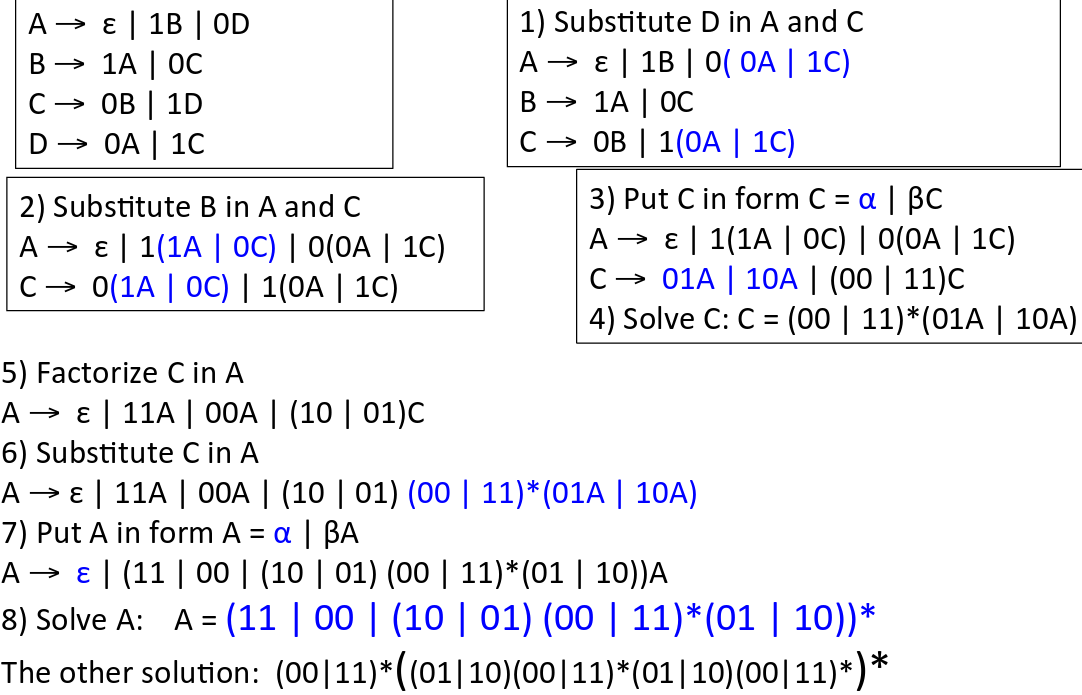
\includegraphics[scale=0.5]{res/image/example_p_re}
  \caption{Esempio ottenimento RE dalla produzione}
  \label{img:example_p_re}
\end{figure}

\subsection{Top-down Parsing}
La sintassi di un programma \`e tipicamente definita da due grammatiche:
\paragraph{Lexical Grammar}
Definisce i \textbf{token}
\begin{itemize}
\item grammatica regolare; presentata come \textit{regular expression}
\item simboli terminali sono caratteri
\end{itemize}
\paragraph{Syantax grammar}
Definisce i \textbf{costrutti del linguaggio}
\begin{itemize}
\item grammatica libera dal contesto; presentata come \textit{Backus-Naur form}
\item simboli terminali sono token
\end{itemize}

Nota: ci sono costrutti sintattici non liberi dal contesto
\begin{itemize}
\item variabili dichiarate prima dell'uso $\to \{wcw \mid w \in (a|b)^*\}$
\item numero di parametri attuali/formali $\to \{a^nb^mc^nd^m \mid n>0,m>0\}$
\end{itemize}

\subsubsection{Towards parsing}
Il parsing implementa la grammatica non libera dal contesto come un
riconoscitore di stringhe:
\begin{enumerate}
\item controlla che la stringa in input (dei token) sia generata dalla
grammatica della sintassi
\item genera il possibile albero di parsing
\item riporta gli errori sintattici accurati
\item invoca le \textbf{azioni semantiche}
\end{enumerate}

le azioni saranno per il controllo statico della semantica (es. type
checking di espressioni, funzioni, ecc.) e per \textit{syntax-directed
translation} dal codice sorgente ad una rappresentazione intermedia.

\paragraph{Descrizione}
Propriet\`a del parsing top-down:
\begin{itemize}
\item accetta CFG ma con restrizioni
\item usa metodi LL (Left-to-right, Leftmost derivation)\footnote{forse vogliono
dire la stessa cosa}
\item complessit\`a \textbf{lineare}
\end{itemize}

Il top-down parsing \`e efficiente se la grammatica soddisfa alcune condizioni:
\textit{quando bisogna espandere i non-terminali, i successivi \textbf{k} token
dovrebbero determinare la produzione da usare} (lookahead). In questo caso la
grammatica \`e $LL(k)$.

\begin{definition}[Left-recursive]
Una grammatica si dice ricorsiva a sinistra se c'\`e un non-terminale $A
\mid A \Rightarrow^+ A\eta$ per qualche stringa $\eta$.
\end{definition}

Nota che la ricorsione a sinistra pu\`o essere indiretta. Una grammatica
ricorsiva a sinistra \textbf{non pu\`o essere} $LL(k)$, per alcuni input il
top-down parser andrebbe in loop.

\subsubsection{Eliminazione ricorsione a sinistra}
Data la grammatica $M$ con la produzione $P$
$$A \to A\alpha | A\beta |  \gamma | \delta$$
per ricondurla ad un'altra grammatica equivalente $M'$ bisogna:
\begin{enumerate}
\item creare un'ulteriore produzione ($A_R$) dove portare tutti terminali
preceduti dal ricorsione
\item nella prima produzione ($A$) affiancare a \textbf{destra} ad ogni
terminale rimasto la produzione creata
\item nella nuova produzione ($A_R$) affiancare a \textbf{destra} la produzione
nuova (ricorsione a destra) e inserire il terminale $\epsilon$
\end{enumerate}

\begin{align}
A   & \to \gamma A_R | \delta A_R \\
A_R & \to \alpha A_R | \beta A_R | \epsilon
\end{align}

Nel caso di produzioni multiple, ove un non-terminale con ricorsione sinistra
appare pu\`o apparire in altre produzioni, \`e necessario eseguire il seguente
algoritmo:

\begin{figure}[H]
\begin{center}
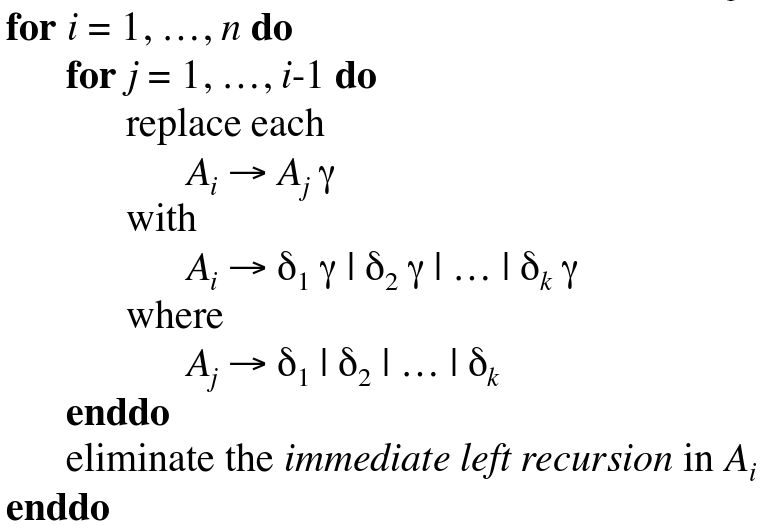
\includegraphics[scale=0.4]{res/image/elimination_Rleft}
\end{center}
\caption{Algoritmo eliminazione ricorsioni sinistre}
\label{img:eliminination_Rleft}
\end{figure}

Il ciclo principale dell'algoritmo prende lista delle produzioni
\textbf{ordinate a scelta}, inizia con le espansioni della produzione (fissata
da $i$) nelle produzioni precedenti (scorse da $j$), e chiude con
\textit{"eliminate the immediate left recursion"} ovvero la procedura spiegata
sopra.

\begin{figure}[H]
\begin{center}
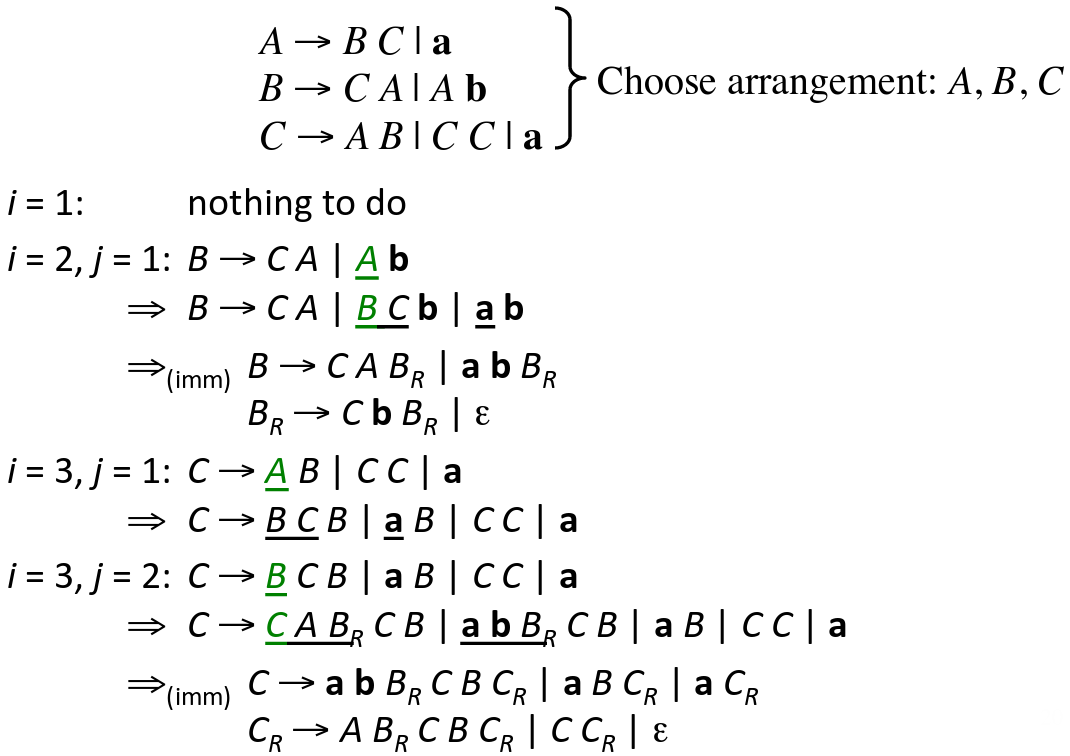
\includegraphics[scale=0.3]{res/image/elimination_example}
\end{center}
\caption{Esempio procedura d'eliminazione}
\label{img:eliminination_example}
\end{figure}

\subsubsection{Elementi del parsing predittivo}
Primo modificare la grammatica in modo che possa essere $LL(1)$, ovvero:
\begin{itemize}
\item eliminazione delle ricorsioni sinistre
\item \textit{left factor} della grammatica
\end{itemize}

successivamente si va a calcolare il \textit{FIRST} ed il \textit{FOLLOW} della
grammatica ed eseguire un ulteriore \textbf{controllo} se la grammatica si
$LL(1)$. Ora si potr\`a eseguire il parsing scegliendo tra:
\begin{itemize}
\item \textbf{Non-recursive} (table-driven parsing)
\item \textbf{Recursive} (recursive-descent parsing)
\end{itemize}

\subsubsection{FOLLOW}
\begin{definition}[Follow]
Il $FOLLOW(A)$ \`e l'insieme dei terminali che possono immediatamente seguire
il non-terminale $A$. Inoltre:
\begin{itemize}
\item $FOLLOW(A) =$
\begin{figure}[H]
\begin{center}
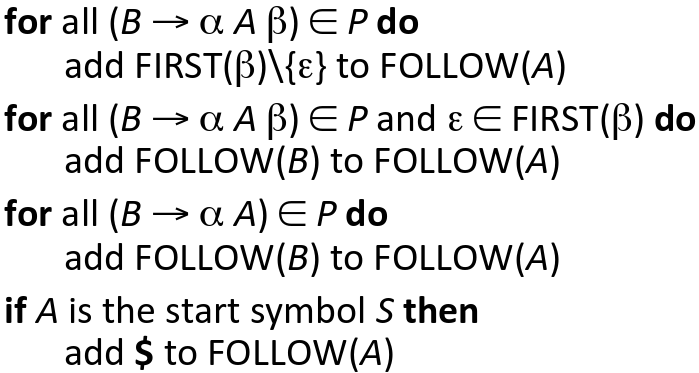
\includegraphics[scale=0.5]{res/image/follow}
\label{img:follow}
\end{center}
\end{figure}
\end{itemize}
\end{definition}

\subsubsection{Grammatiche LL(1)}
\begin{definition}[LL(1) grammar]
Una grammatica $G$ si dice $LL(1)$ se \textbf{non c'\`e} ricorsione sinistra e
per ogni collezione di produzioni
$$A \to \alpha_1|\alpha_2|...|\alpha_n$$
per il non-terminale $A$ la seguenti condizioni:
\begin{enumerate}
\item $FIRST(\alpha_i) \cap FIRST(\alpha_j) = \emptyset \quad \forall i \neq j$
\item $\text{if } \alpha_i \Rightarrow^* \epsilon \text{ then}$
\begin{enumerate}
\item $a_j \not{\Rightarrow^*} \epsilon \quad \forall i \neq j$
\item $FIRST(\alpha_j) \cap FOLLOW(A) = \emptyset \quad \forall i \neq j$
\end{enumerate}
\end{enumerate}
\end{definition}

La seguente tabella mostra alcuni esempio di grammatiche non $LL(1)$:
\begin{figure}[H]
\begin{center}
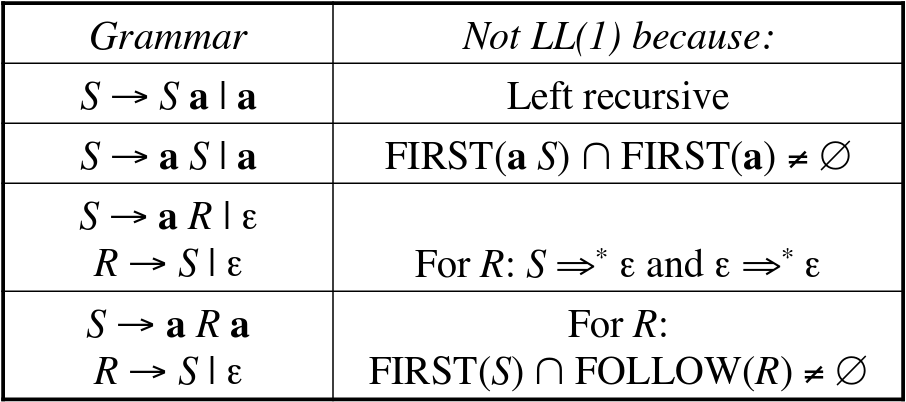
\includegraphics[scale=0.5]{res/image/no_LL1}
\end{center}
\caption{Esempio di grammatiche no $LL(1)$}
\label{img:en_LL1}
\end{figure}

\subsubsection{Parsing ricorsivo discendente}
La costruzione dell'algoritmo di \textit{Recursive-Descent Parser} \`e molto
semplice:
\begin{itemize}
\item ogni \textbf{non-terminale} ha una \textbf{procedura} (ricorsiva)
responsabile per eseguire il parsing della categoria sintattica dei terminali,
gli input token
\item quando un non-terminale ha produzioni multiple ogni \textbf{produzione}
\`e implementata in un \textbf{branch} basato sull'informazione del
\textit{lookahead}
\end{itemize}

Esempio mostra come vengono utilizzati il $FIRST$ ed il $FOLLOW$ (va usato solo
quando si incappa in una $\epsilon$-produzione) durante la
fase di parsing:
\begin{figure}[H]
\begin{center}
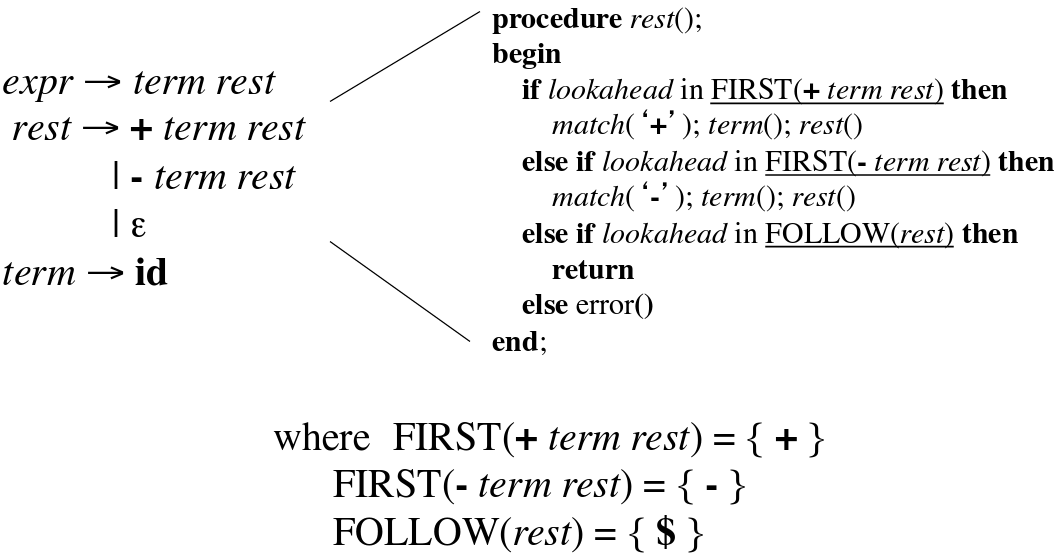
\includegraphics[scale=0.4]{res/image/example_RDP}
\end{center}
\caption{Dalla grammatica al codice per il parsing ricorsivo discendente}
\label{img:example_RDP}
\end{figure}

Nota: la grammatica \textbf{deve} essere $LL(1)$.

\subsubsection{Parsing non-ricorsivo predittivo}
L'eliminazione della ricorsione avviene mediante una tabella $M$ costruita a
partire dalla grammatica $LL(1) G=(N,T,P,S)$ tramite un programma
\textit{driver} con uno \textit{stack}. Quest'ultimo va a rimpiazzare lo stack
a \textit{runtime} dell'algoritmo ricorsivo, tenendo i simboli della grammatica.

\begin{figure}[H]
\begin{center}
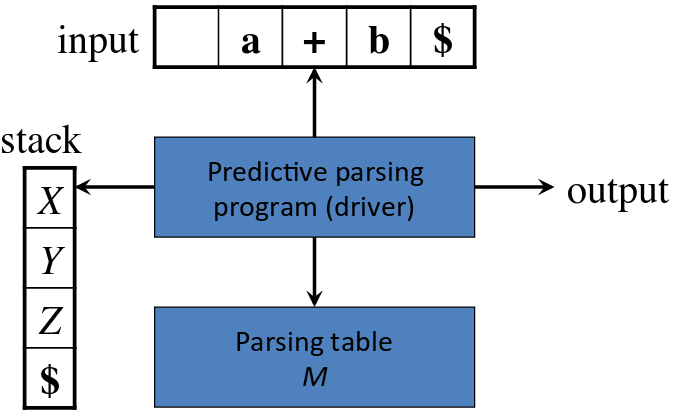
\includegraphics[scale=0.5]{res/image/driver_stack}
\end{center}
\caption{Rappresentazione \textit{driver} con \textit{stack}}
\label{img:driver_stack}
\end{figure}

\subsubsection{Costruzione della Predictive Parsing Table}
Data la grammatica $G=(N,T,P,S)$ si ha una tabella $M$ con:
\begin{itemize}
\item un entry $M[A,a]$ per ogni $A \in N$ e $a \in T$
\item la entry $M[A,a]$ contiene le produzioni da applicare ad $A$ quando \`e
stata ridotta e $a$ \`e il suo \textit{lookahead}
\item ogni entry \textbf{indifenita} in $M$ \`e marcata come errore
\end{itemize}

La grammatica \`e $LL(1)$ sse $M[A,a]$ contiene al pi\`u una produzione $\forall
A \in N$ e $a \in T$. Dai passi indicati si deriva l'algoritmo per la creazione
della tabella $M$:

\begin{figure}[H]
\begin{center}
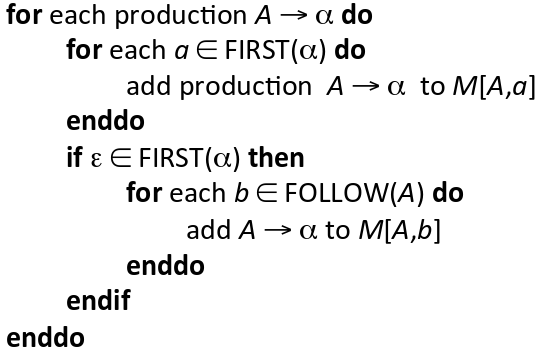
\includegraphics[scale=0.5]{res/image/algorithm_fill_M}
\end{center}
\caption{Algoritmo riempimento tabella $M$}
\label{img:algorithm_fill_M}
\end{figure}

L'immagine \ref{img:example_create_M} \`e un esempio di come viene creata la
tabella $M$. Prima si produce una tabella intermedia dove si individua il
$FIRST$ ed il $FOLLOW$ dei vari non-terminali; se un non-terminale ha produzioni
multiple si dividono. Una volta completata si applica l'algoritmo di
fig.\ref{img:algorithm_fill_M}

\begin{figure}[H]
\begin{center}
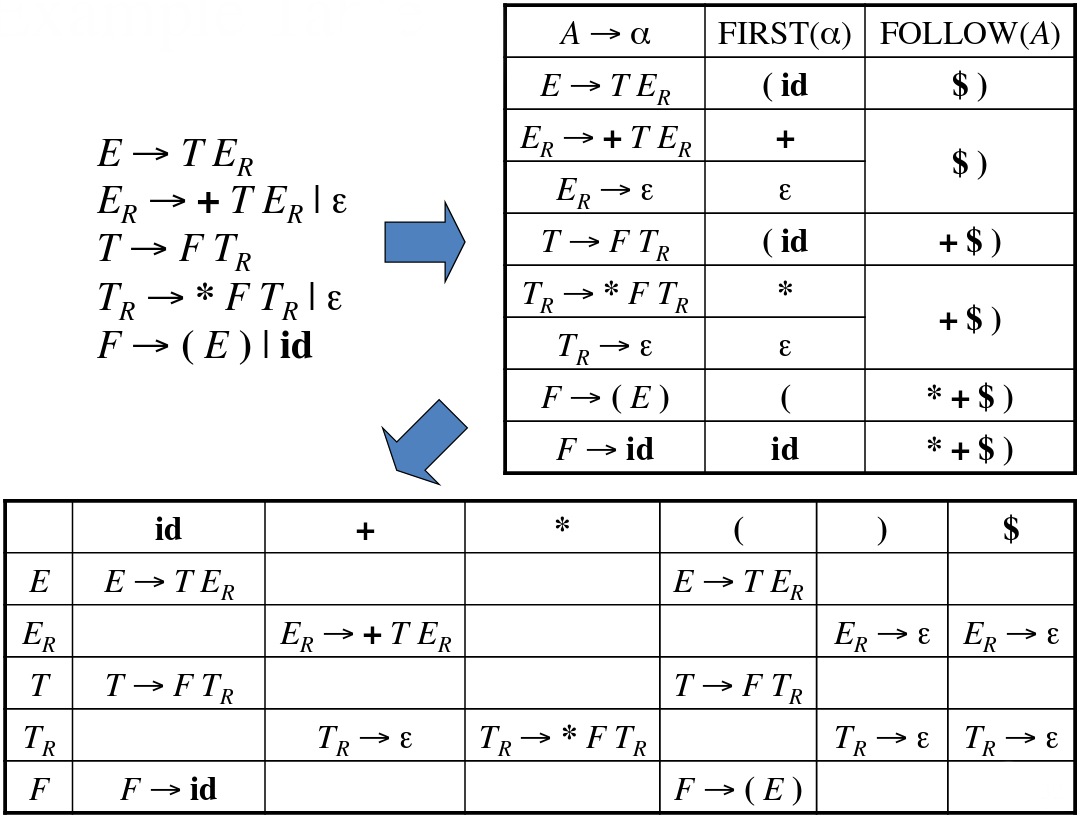
\includegraphics[scale=0.3]{res/image/example_create_M}
\end{center}
\caption{Esempio creazione tabella $M$}
\label{img:example_create_M}
\end{figure}

Se la grammatica nel quale si tenta di costruire la tabella $M$ \`e
\textbf{ambigua} si otterrebbe che per alcune entry della tabella vengono
inserite pi\`u produzioni. La figura sottostante ne mostra un esempio.

\begin{figure}[H]
\begin{center}
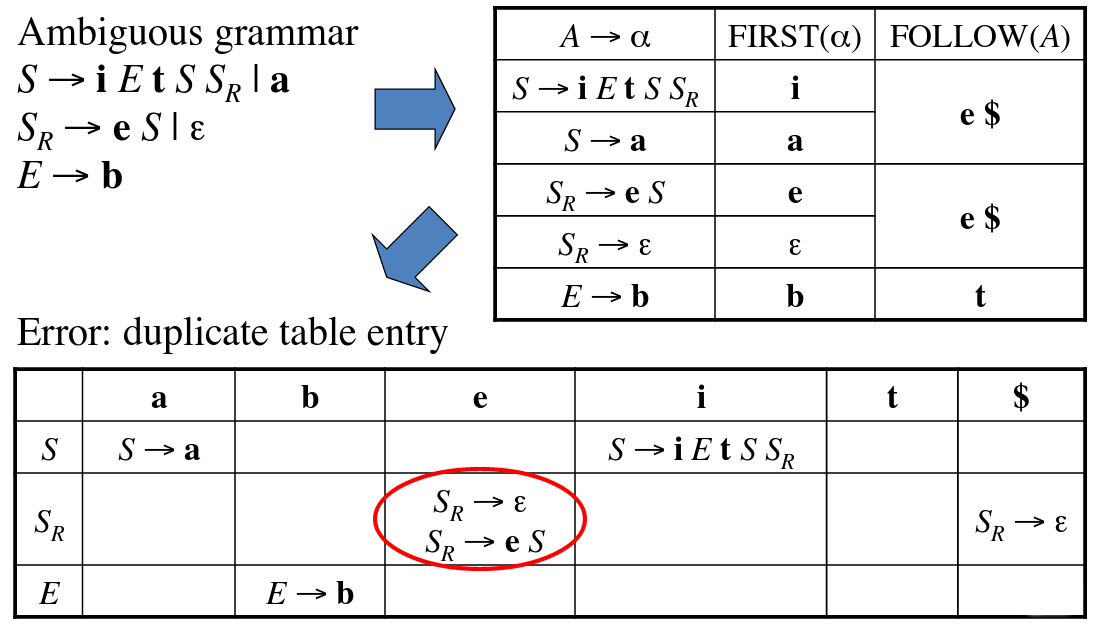
\includegraphics[scale=0.3]{res/image/conflict_in_M}
\end{center}
\caption{Esempio conflitti $M$ per grammatica ambigua}
\label{img:conflict_in_M}
\end{figure}

\subsubsection{Programma di parsing predittivo}
Una volta creata la tabella il \textit{Predictive Parsing Program}
(o \textit{Driver}) pu\`o utilizzarla per eseguire l'espansione dei
non-terminali e di conseguenza eseguire le azioni associate (es. generare la
rappresentazione intermedia). L'algoritmo \`e quello in fig.\ref{img:PPP}.

\paragraph{Inizializzazione - \textit{l.0-2}}
si va ad inserire nello stack il primo simbolo (\$) il quale sar\`a l'ultimo ad
essere elaborato: il raggiungimento di quel simbolo nello stack determina la
buona riuscita del parsing. Successivamente si mette in testa il primo
non-terminale con cui iniziale la ricerca e si setta il \textit{lookahead} al
primo simbolo dell'input.

\paragraph{Estrazione - \textit{l.4}}
\label{par:extraction}
preleviamo simbolo nel top dello stack. Da qui il comportamento del programma
dipender\`a se il simbolo \`e un terminale o un non-terminale. Se fosse un
non-terminale si avrebbe la chiave della riga $M$ in corrispondenza del simbolo
$A$.

\paragraph{Se terminale - \textit{l.5-6}}
\label{par:if_terminal}
Le continue espansioni dei non-terminali nello stack hanno portato ad avere un
terminale. Qui si procede con il \textit{match} del terminale con quello atteso
(vedere funzione match) e se \`e positivo si consuma l'attuale \textit{lookahed}
passando a quello successivo.

\paragraph{Se non-terminale - \textit{l.7-9}}
\label{par:if_non-terminal}
Il \textit{lookahead} fornisce il simbolo che determina la colonna di $M$.
Attraverso la coppia $(A,a)$ (in questo caso $A=X$) si va ad espandere il
non-terminale. I simboli sono inseriti al contrario in modo da non perdere
l'ordine dato dallo stack. Da qui invochi azioni o produci la
\textit{Intermediate Rappresentation} (IR).

\paragraph{Loop e fine}
La procedura d'estrazione e controlli avviene fin tanto che non si \`e tornati
al simbolo \$ inserito nel bottom dello stack durante l'inizializzazione. Se
il simbolo estratto non soddisfasse le condizioni dei due branch allora si \`e
incappati in un errore.

\begin{figure}[H]
\begin{center}
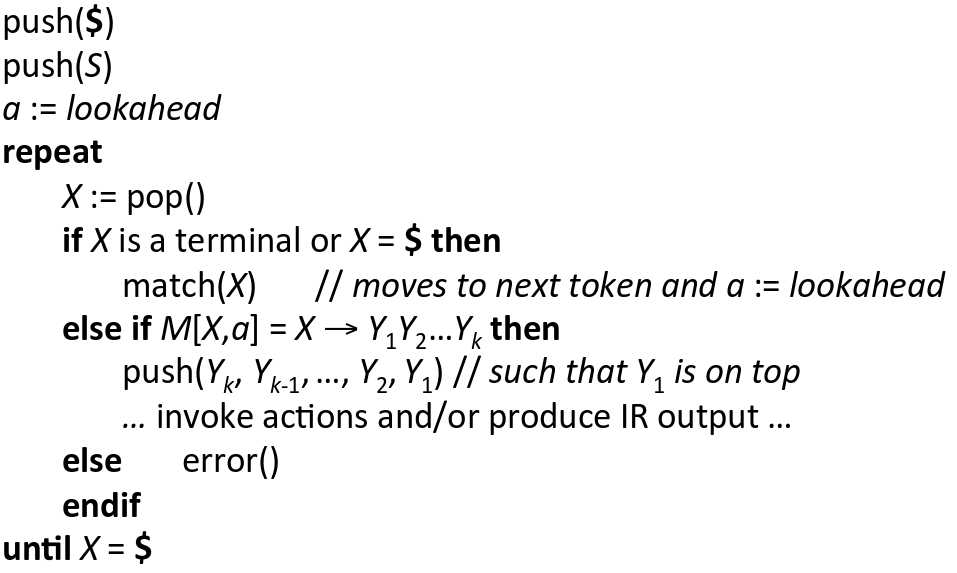
\includegraphics[scale=0.45]{res/image/PPP}
\end{center}
\caption{Algoritmo del parsing predittivo}
\label{img:PPP}
\end{figure}

\subsection{Gestione errori}
Un buon compilatore dovrebbe assistere nell'identificazione e localizzazione
degli errori.

\begin{table}[H]
\begin{center}
\begin{tabular}{|c|p{6cm}|p{4cm}|}
\hline
\textbf{Errore} & \textbf{Identificazione} & \textbf{Esempio} \\ \hline
\textit{Errori lessicali} &
Facile, recupero e proseguimento possibile &
Errore ortografico \\ \hline
\textit{Errore sintattico} &
Quasi sempre recuperabili &
";" o "\}" mancante, "case" smarrito \\ \hline
\textit{Errori semantici statici} &
Qualche volta recuperabili &
Tipi incompatibili, dichiarazione prima dell'uso \\ \hline
\textit{Errori semantici dinamici} &
Difficile o impossibile a \textit{compile-time} &
Puntatore \textit{NULL}, divisione per zero, accesso errato array \\ \hline
\textit{Errori logici} &
Difficile o impossibile &
\textit{if (b \textbf{=} true) ...} \\ \hline
\end{tabular}
\end{center}
\caption{Tabella errori di compilazione}
\label{tab:compiler_error}
\end{table}

\subsection{Error Detection Strategy}
\subsubsection{Viable-Prefix Property}
La \textit{Viable-Prefix Property} dei parser permette l'identificazione degli
\textbf{errori di sintassi}.

\paragraph{Grammatica}
funziona con parser \textit{LL(1)} ed \textit{LR(1)}.
\paragraph{Obiettivo}
individuazione degli errori il pi\`u presto possibile senza consumare input
distanti non necessari.
\paragraph{Come}
individua un errore appena un prefisso dell'input non coincide con \textbf{i
prefissi di ogni stringa} nel linguaggio.

\subsection{Error Recovery Strategies}
\subsubsection{Panic Mode Strategy}
chiamati \textit{synchronizing tokens} \`e trovato (es. "\}", ";").
Scarta elementi in input finch\'e un token in un insieme di token designati

La realizzazione avviene trammite l'aggiunta di un'azione \textit{synch} per
le entry nella tabella $M$ \textbf{indefinite} basate sul $FOLLOW$. Ci\`o
significa che nella riga di $A$ inserir\`o un'azione di sincronizzazione nelle
entry corrispondenti ai terminali nell'insieme del $FOLLOW(A)$, se sono vuote.

\begin{figure}[H]
\begin{center}
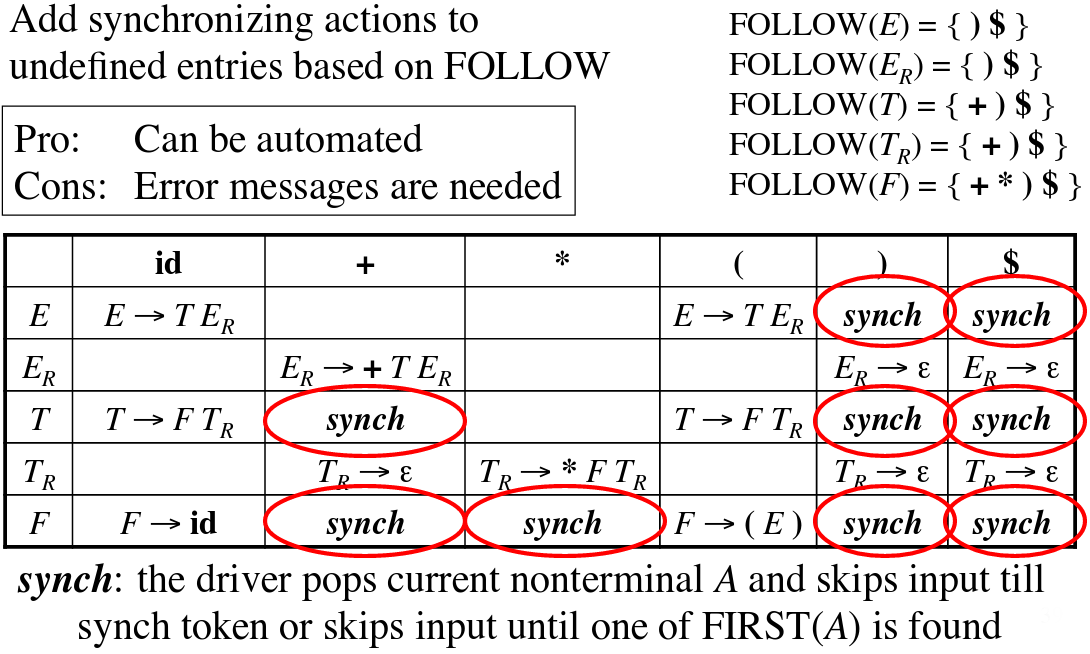
\includegraphics[scale=0.35]{res/image/example_panic_mode}
\end{center}
\caption{Esempio completo del \textit{Panic Mode}}
\label{img:example_panic_mode}
\end{figure}

Nell'esempio sopra si pu\`o notare che la posizione del \textit{synch} coincide
con la posizione dei terminali appartenente al $FOLLOW$ dei vari non-terminali.
L'azione \textit{synch} comanda al driver di fare il pop del non-terminale $A$
(quello in testa allo stack in attesa di essere espanso) e ignora i simboli in
input finch\'e o trova un terminale \textit{synch} o trovi un $FIRST(A)$.

\subsubsection{Phrase-level recovery}
\label{sec:phrase-level_recovery}
Applica una correzione \textbf{locale} sull'input per riparare l'errore.
Si attua questo correzione inserendo un'azione (es. \textit{insert*}) in
corrispondenza di una entry indefinita di $M$.

\begin{figure}[H]
\begin{center}
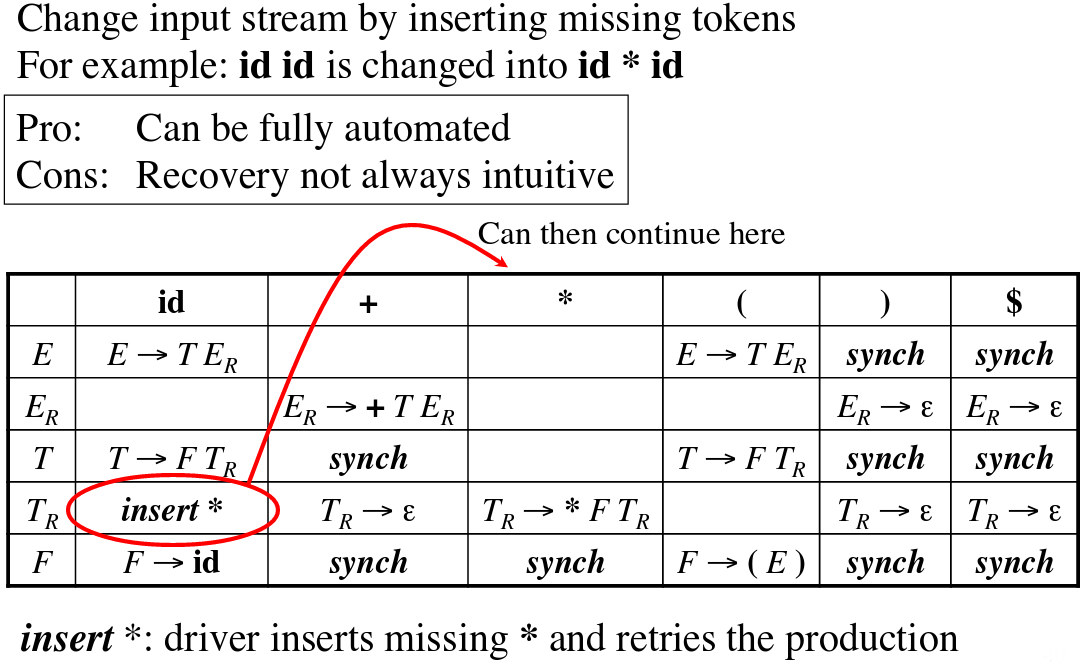
\includegraphics[scale=0.35]{res/image/example_phrase_level}
\end{center}
\caption{Esempio completo del \textit{Phrase-level}}
\label{img:example_phrase_level}
\end{figure}

\subsubsection{Error productions}
Aumenta la grammatica con produzioni per erronee costruzioni.

\begin{figure}[H]
\begin{center}
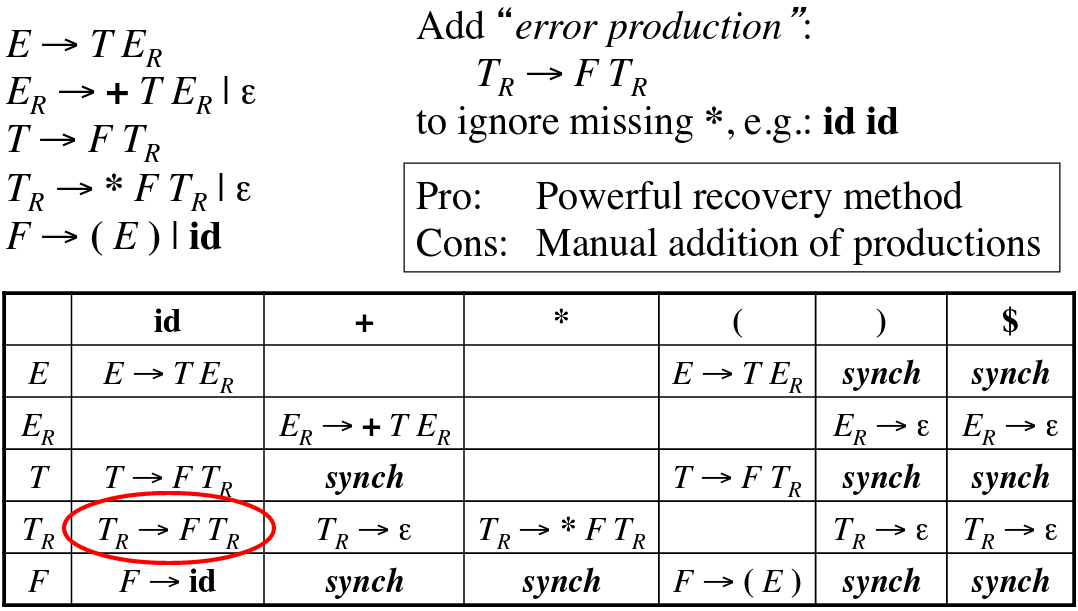
\includegraphics[scale=0.4]{res/image/example_error_productions}
\end{center}
\caption{Esempio completo dell'\textit{Error Productions}}
\label{img:example_error_productions}
\end{figure}


\subsubsection{Global correction}
Scegli una \textbf{minima} sequenza di cambiamenti per ottenere una globale
correzione a costo minimo.
